\documentclass{article}
\usepackage{fullpage}
\usepackage{verbatim}
\usepackage{graphicx}
\usepackage{hyperref}
\usepackage{pdflscape}


\begin{document}
\title{Software Architecture}
\author{Chiel Peters, Omar Pakker, Mary Gouseti, Cindy Berghuizen}
\maketitle
\setlength\parindent{0pt}
\section{Definition of Architecture}

First four definitions of software architecture are stated and their differences
and similarities are discussed. Second, our own view on software architecture is
given.
\subsection{Definitions on architectures}

\begin{enumerate}
\item Software Architecture is the set of structures needed to reason about the software system, which comprise the software elements, the relations between them, and the properties of both elements and relations.\cite{clemens}

\item Software Architecture is an abstract system specification consisting primarily of functional components described in terms of their behaviours and interfaces and component-component interconnections\cite{hayesroth}

\item Software Architecture is the fundamental organization of a system embodied in its components, their relationships to each other, and to the environment, and the principles guiding its design and evolution.\cite{IEEE1471}

\item Software architecture is the study of the large-scale structure and performance of software systems. Important aspects of a system's architecture include the division of functions among system modules, the means of communication between modules, and the representation of shared information.\cite{lane90}

\end{enumerate}

These definitions share the same fundamental idea that software architecture
is a set of structures/components/modules including their properties and the
relationships between them. However, each of the definitions highlights certain
aspects of architecture more than the others. 
\begin{itemize}
\item In \cite{clemens} and \cite{hayesroth} the focus has been put on the end result. The architecture 
is defined as the components themselves (their properties/interfaces) and the relationships between them (interconnections).
\item The definition stated in \cite{hayesroth} lays a focus on the functional components of a software architecture. With words like functional components, 
behaviours and interfaces underlines the importance of declaring the way the components interact with each other.
\item The definition of \cite{IEEE1471} is limited only to the systems components and their functionalities and connections but also includes in the definition the 
process of designing and maintaining an architecture. It explicitly states that the design process and the evolution are part of the architecture itself.
\item The last definition (\cite{lane90}) presents architecture as the study a system's structure. As a result architecture contains the modules and the connections between them that build the system. This also becomes clear
from the title of the article \emph{Studying Software Architecture Through Design Spaces and Rules}.

\end{itemize}

\subsection{Our view on architecture}
As the definitions mentioned above, we also agree on the point that a software architecture is defined as a set of components, their properties, behaviours and the relations
between. However, we think that architecture is not only the structure of a software system but also contains the main design decisions that would explain why the system consists of 
these components and include the stakeholders' quality attributes that lead the architects to those decisions. \\ 

Our definition of software architecture would be:
Software architecture is the structure of a software system along with the decisions that lead to this structure. To elaborate architecture contains the components by which
the system is build up, their functionality, the relations between them and the reason of their existence meaning which requirement of the stakeholders or quality attribute they accomplish. 
%stakeholderpart
\section{Stakeholder Concerns}

In this project there are four different stakeholder :
\begin{enumerate}
\item The Initiator
\item AirFrance - KLM
\item The Dutch Government
\item EU Claim
\end{enumerate}

Each of them had different concerns within this project which are stated in the next subsections.

\subsection{Initiator}
The initiator is the one who started this project. He wants FlyWithUs to be a success and become the number one rating site people will go to. He want to be able to collect data from social media, other rating websites, news, weather and every other source that can be of importance. This data an then be used to provide the airlines with powerfull statistics and can give users a final rating. Users that make use of FlyWithUs have to be able to post reviews and ratings on the website and search for them. What makes FlyWithUs unique is the fact that airlines can get in touch with the users by sending them messages.

\subsection{AirFrance - KLM}
This stakeholder wants to have a reporting tool. With the tool he has to be able to see what recent reviews have been posted about his airline. Also, AirFrance - KLM wants to see statistics and be able to see what causes a sudden decline or increase in the rating. Furthermore, AirFrance-KLM wants to be able to enter flight information and by doing so influence the weight of review. This means that the weight of a rating has to be less when bad ratings are due to for example environmental issues (bad weather etc.) and have nothing to do with the airline companies services.

\subsection{Dutch Government}
Privacy is an important issue for the Dutch Government. The server needs to be hosted in the Netherlands so FlyWithUs will be led according to the Dutch Privacy Law. Also, the Dutch Governemnt would like to see the project to be a "Green IT" project. 

\subsection{EU Claim}
EU Claim wants to make certain that the privacy if the user is guaranteed. Furthermore the airlines have to behave on the website and do not mess with the results or bribe the users. Fairness is thus also an important issue to this stakeholder.

%Input viewpoints here
\section{Viewpoints}
% % % \input{PrivacyView}

\subsection{Privacy viewpoint}

\begin{itemize}
\item Related stakeholders: Dutch government, EU Claim
\item Related Concerns: Privacy of the user
\end{itemize}

\newpage
\begin{landscape}
\begin{figure}
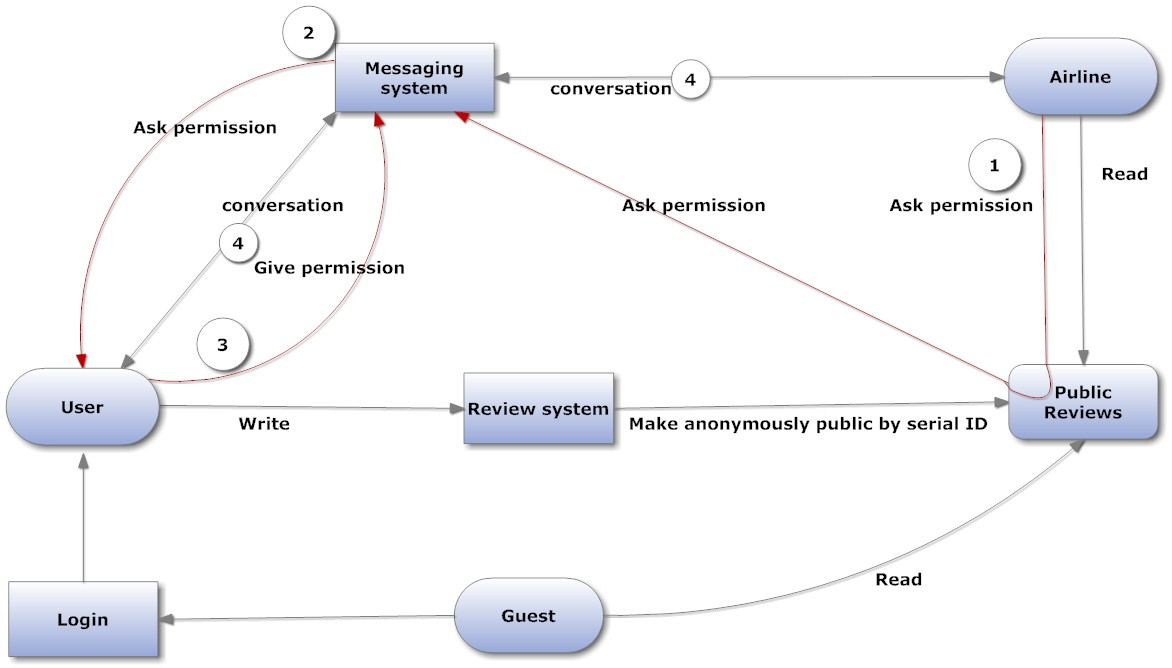
\includegraphics[width=680px]{privacyview}
\caption{Privacy viewpoint}
\label{fig:privacy}
\end{figure}
\end{landscape}
The privacy viewpoint in figure \ref{fig:privacy} shows how the privacy of the user is guaranteed in the system. A user can write a review that is shown to the public anonymously. The review will have a serialID instead of the user name so the user will stay unknown to the public. 

An airline should be able to have a conversation with an user if the airline wants to elaborate on a specific case or wants to adress the user personally. If the airline wants to get the user's information for a conversation it should ask permission of the user. When a user accepts to have a conversation with an airline the user's contact information is visible to the airline so they will be able to have a conversation. If the user is not satisfied with how the airline company responds on requests or remarks in the conversation, the user is able to invite EU Claim to the conversation so they will be able to see the conversation and decide to act upon it.

\subsection{Privacy viewpoint}

\begin{itemize}
\item Related stakeholders: Dutch government, EU Claim
\item Related Concerns: Privacy of the user
\end{itemize}

\newpage
\begin{landscape}
\begin{figure}
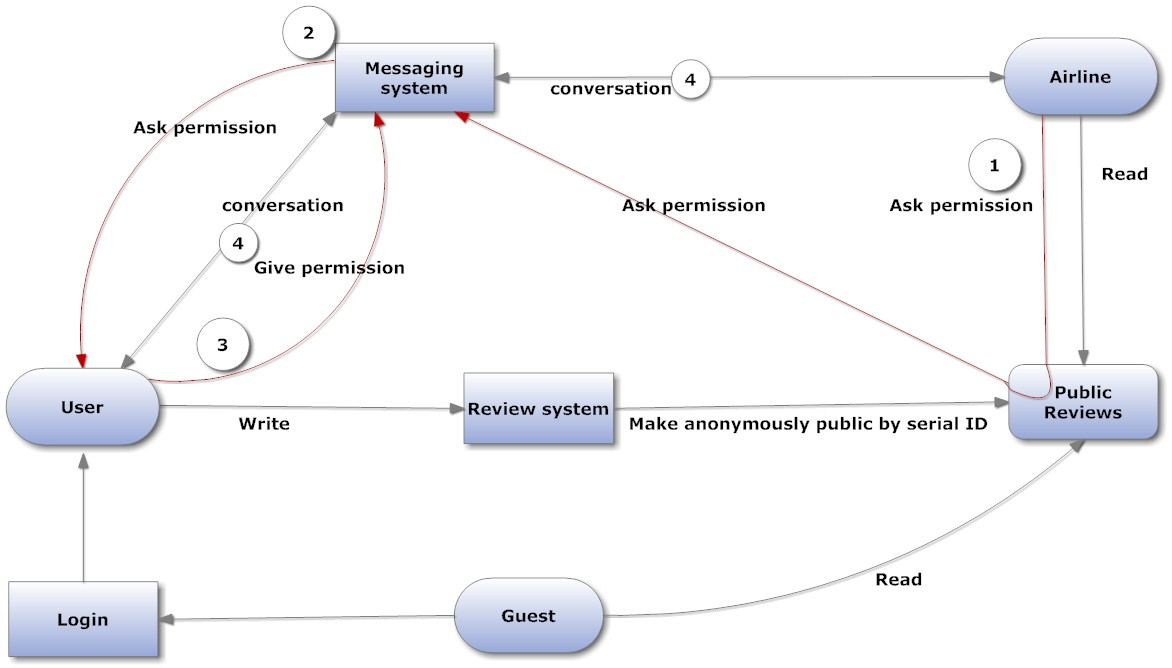
\includegraphics[width=680px]{privacyview}
\caption{Privacy viewpoint}
\label{fig:privacy}
\end{figure}
\end{landscape}
The privacy viewpoint in figure \ref{fig:privacy} shows how the privacy of the user is guaranteed in the system. A user can write a review that is shown to the public anonymously. The review will have a serialID instead of the user name so the user will stay unknown to the public. 

An airline should be able to have a conversation with an user if the airline wants to elaborate on a specific case or wants to adress the user personally. If the airline wants to get the user's information for a conversation it should ask permission of the user. When a user accepts to have a conversation with an airline the user's contact information is visible to the airline so they will be able to have a conversation. If the user is not satisfied with how the airline company responds on requests or remarks in the conversation, the user is able to invite EU Claim to the conversation so they will be able to see the conversation and decide to act upon it.

\subsection{Privacy viewpoint}

\begin{itemize}
\item Related stakeholders: Dutch government, EU Claim
\item Related Concerns: Privacy of the user
\end{itemize}

\newpage
\begin{landscape}
\begin{figure}
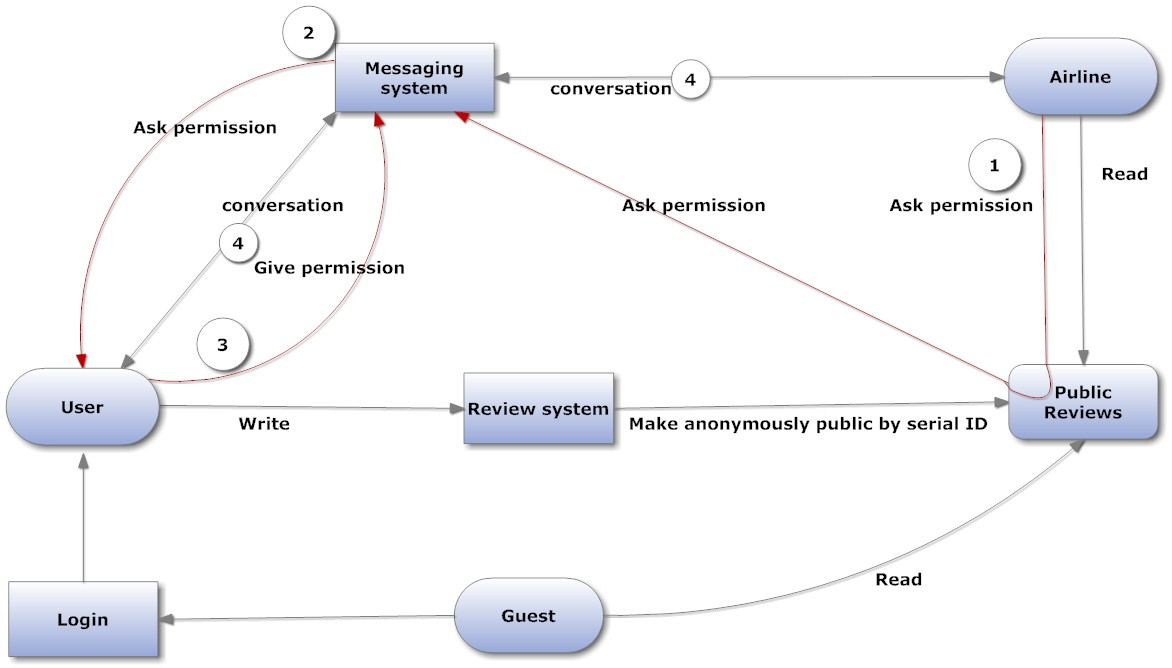
\includegraphics[width=680px]{privacyview}
\caption{Privacy viewpoint}
\label{fig:privacy}
\end{figure}
\end{landscape}
The privacy viewpoint in figure \ref{fig:privacy} shows how the privacy of the user is guaranteed in the system. A user can write a review that is shown to the public anonymously. The review will have a serialID instead of the user name so the user will stay unknown to the public. 

An airline should be able to have a conversation with an user if the airline wants to elaborate on a specific case or wants to adress the user personally. If the airline wants to get the user's information for a conversation it should ask permission of the user. When a user accepts to have a conversation with an airline the user's contact information is visible to the airline so they will be able to have a conversation. If the user is not satisfied with how the airline company responds on requests or remarks in the conversation, the user is able to invite EU Claim to the conversation so they will be able to see the conversation and decide to act upon it.
% % % \input{DataFlow}

\subsection{Data Flow Viewpoint}

\begin{itemize}
\item Related stakeholders: KLM, Initiator
\item Related Concerns: Data Integrity, Performance, Scalability
\item Related design decisions: How is the data split up into multiple databases?; How do we handle large data-sets?; Recalculate or Combine rating?; Incremental or Time-interval update?; Flight-Information
\end{itemize}

\newpage
\begin{landscape}
\begin{figure}
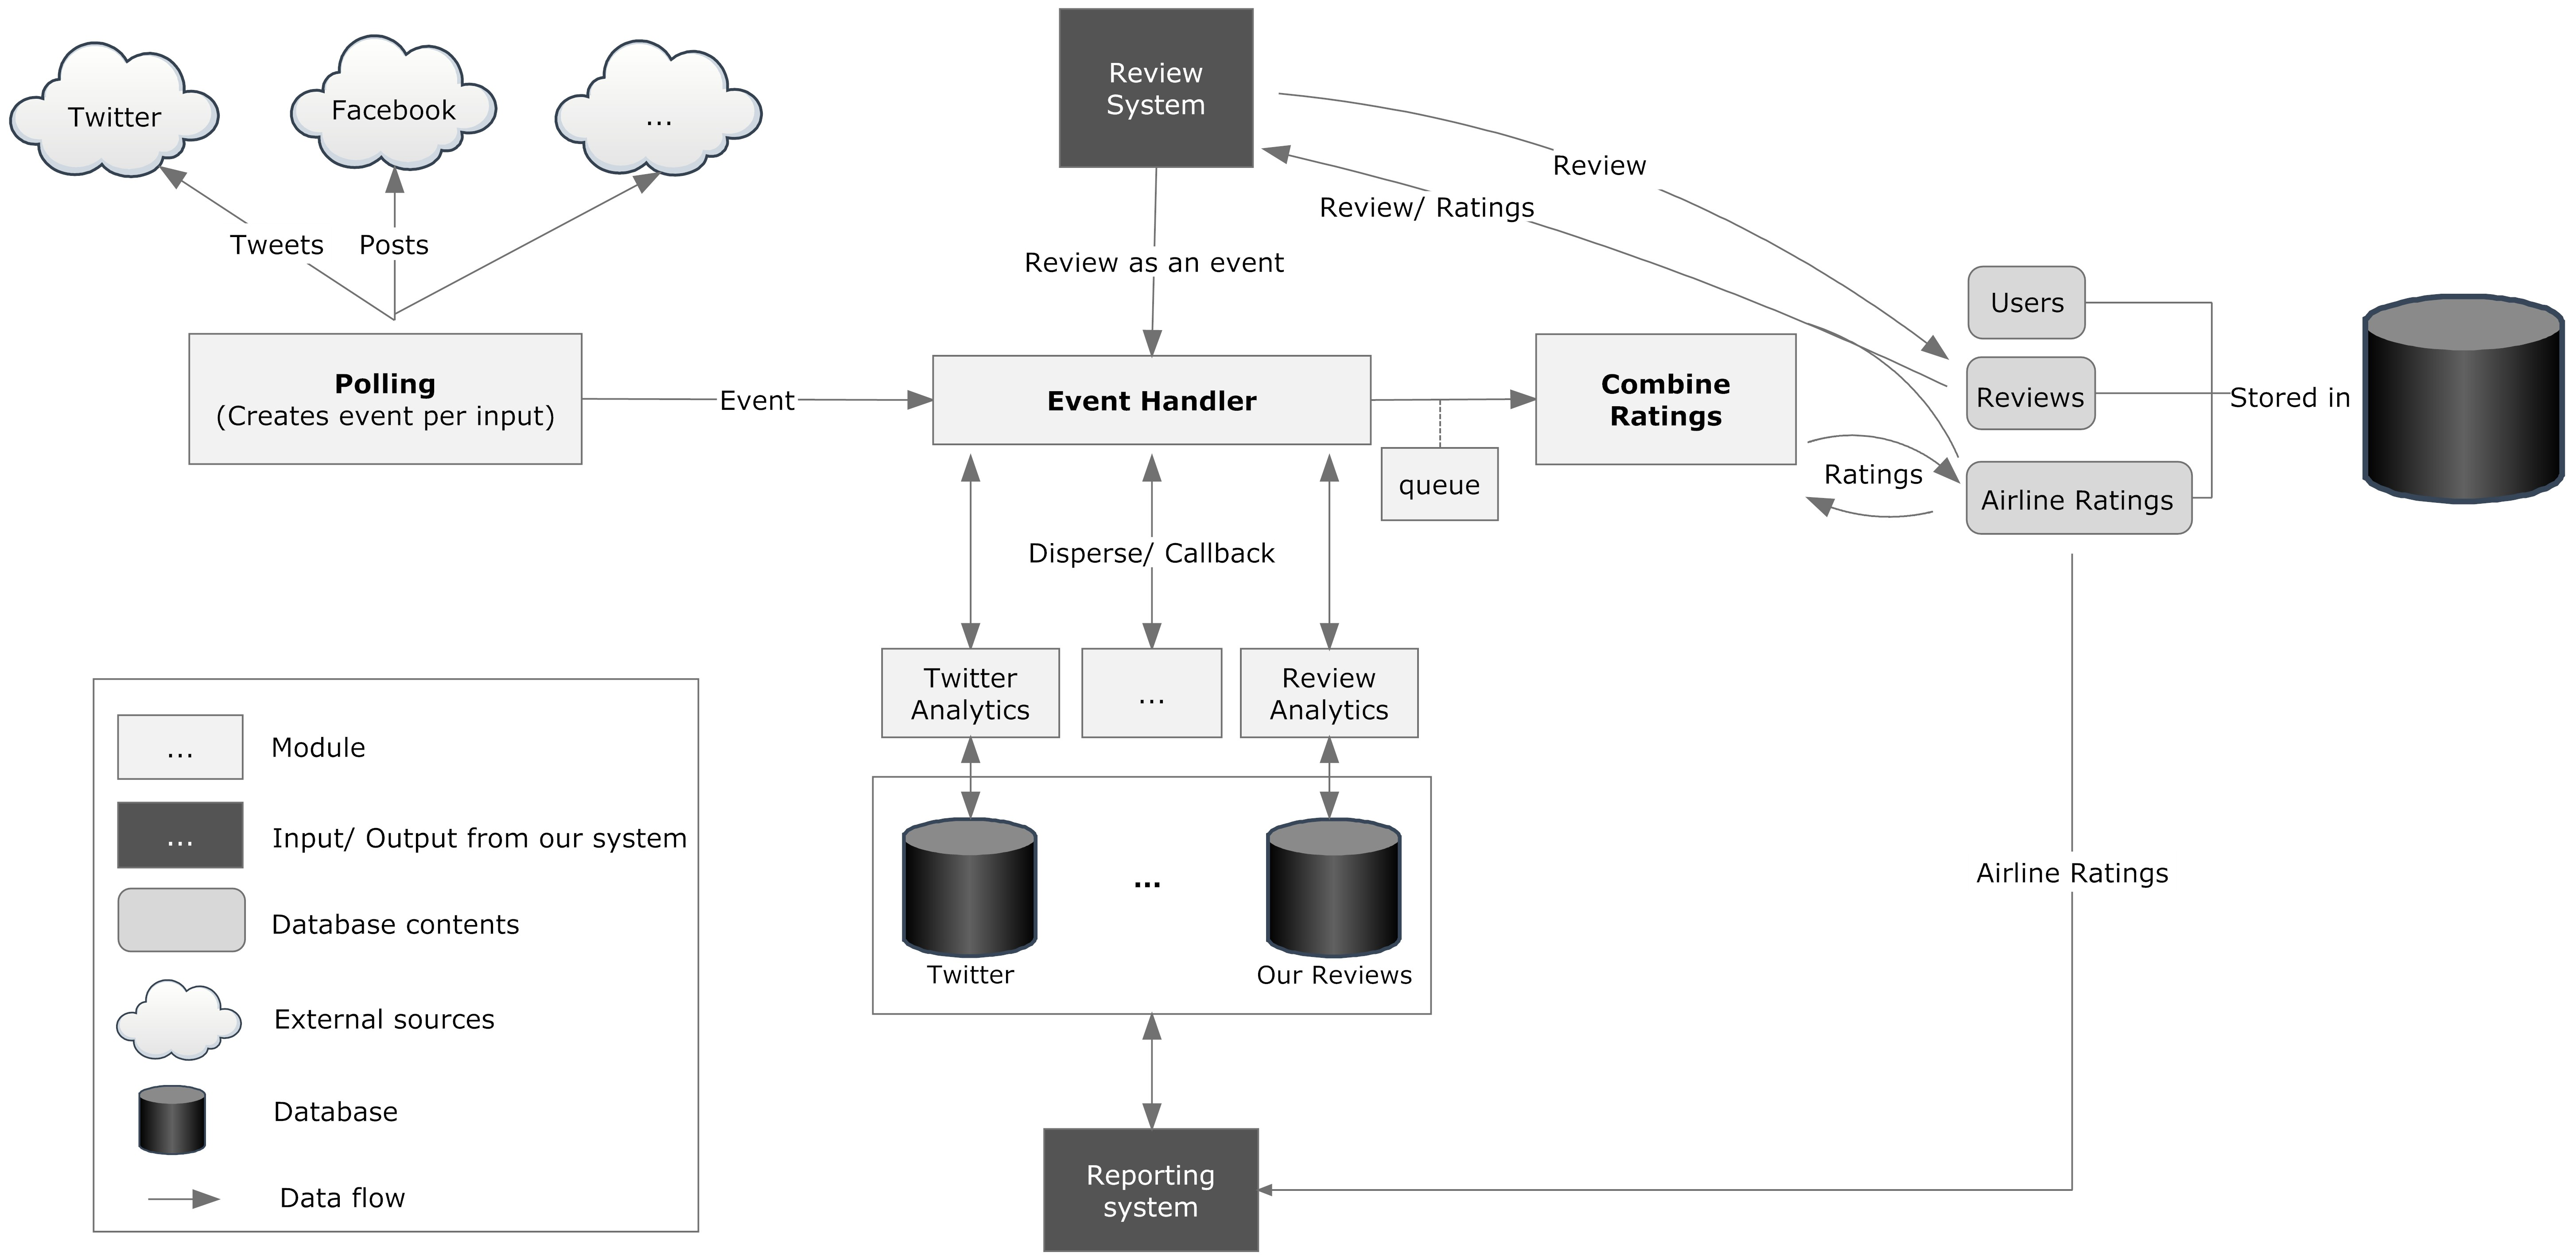
\includegraphics[width=600px]{DataFlowGraph}
\caption{Data Flow Viewpoint}
\label{fig:Data Flow}
\end{figure}
\end{landscape}

This Data Flow viewpoint \ref{fig:Data Flow} illustrates the flow of data within the back-end of the system. In this picture the review and reporting system are shown as black boxes to illustrate that their functionality is of no importance in this picture.
In the related design decisions it was argued that combining the rating with incremental updates was best for performance and scalability. Note that in the flow only the back-end of the system is given, because of the importance of handling the large data sets. Each of the modules and arrows in the viewpoint are explained here after.

\subsubsection{Polling}
The polling module is responsible for obtaining reviews from external data sources. It polls every external source on a given time-frame which is different for each external source. The reviews are not formatted and there original data format from the external source is kept. The rationale behind this decision is that all the reviews from external sources are significantly different of each other. Parsing them into a general format would lead to data loss or lots of undefined fields. The decision is further elaborated in the appendix at \ref{dd:save-raw}. The unformatted reviews are then passed on to the event handler as events. An event is defined as a single unformatted review either from external or internal sources.

\subsubsection{Event handler}
The event handler receives the events from both the polling module (external sources) and the review system (internal source). The responsibility of the event handler is to send these events to the analytics module specific to that data source. The event handler allows for parallel processing of reviews and greatly increased the performance and scalability compared to a more traditional pipeline model. This decision is further elaborated on in the appendix at \ref{dd:large-data}.

\subsubsection{Analytics}
Each data source has its own analytics module, because the data must be treated differently from external sources as they are of different format. The separate analytics modules have the added benefit of allowing for meta-analysis specific to a given data source. An example could be the amount of followers on twitter.

The analytics module analyses the unformatted review and produces a rating on a given scale for a certain or multiple categories (Overall, food, timeliness etc.). The unformatted review together with the analysed ratings are then stored in the analytics database of the data source. This is a requirement by the Initiator and KLM. The decision is further discussed in the appendix \ref{dd:data-format}. The ratings are also send of the combine ratings module in order to update the rating of the airline that is related to the review.

\subsubsection{Combine Ratings}
The combine ratings module is responsible for combining the ratings from the individual reviews into a final rating for an airline. The module receives the ratings from the analytics module and obtains the old rating from the main database. These two are combined in order to form a new rating. The process of iteratively combining ratings instead of recalculating is made for performance reasons as it is much cheaper and efficient to not recalculate the ratings that are already in the final rating of the airline. This decision is discussed in the appendix at \ref{dd:recalc-comb}. The ratings are based on an airline and a specific category (overall, timeliness, food etc.).

\subsubsection{Modules}
The functionality of each of the modules is discussed in the functional view. Hence in this section only the data flow regarding each of the modules is discussed:

\begin{enumerate}
\item \emph{R \& R module} A new review is inserted as event into the event handler which can pass it off to the specific analytics module. The decision was made to save the internal reviews twice: once in the main database and once when the they are analysed in the Analytics database. This allows the users to see the reviews without accessing the analytics database, but increases overhead as the same data is almost saved twice.
\item \emph{Reporting module} The reporting module retrieves information from the analytics database which contain all the analysed data together with the raw reviews. It must also be able to access the main database for the latest final ratings.
\item \emph{Authentication module} The user data for logging purposes is saved in the main database. The data contains sensitive information and is therefore encrypted.
\item \emph{Billing module} In order to make a profit airlines need to pay for their functionality. Therefore the billing module is able to read the current enlisted airlines and write to the database if the airlines have paid or not.
\item \emph{Messaging module} The messages are saved separately in the main database. Because they can contain user sensitive information (e.g. Flight numbers, names) the whole messages are saved in an encrypted form.
\end{enumerate}


\subsection{Data Flow Viewpoint}

\begin{itemize}
\item Related stakeholders: KLM, Initiator
\item Related Concerns: Data Integrity, Performance, Scalability
\item Related design decisions: How is the data split up into multiple databases?; How do we handle large data-sets?; Recalculate or Combine rating?; Incremental or Time-interval update?; Flight-Information
\end{itemize}

\newpage
\begin{landscape}
\begin{figure}
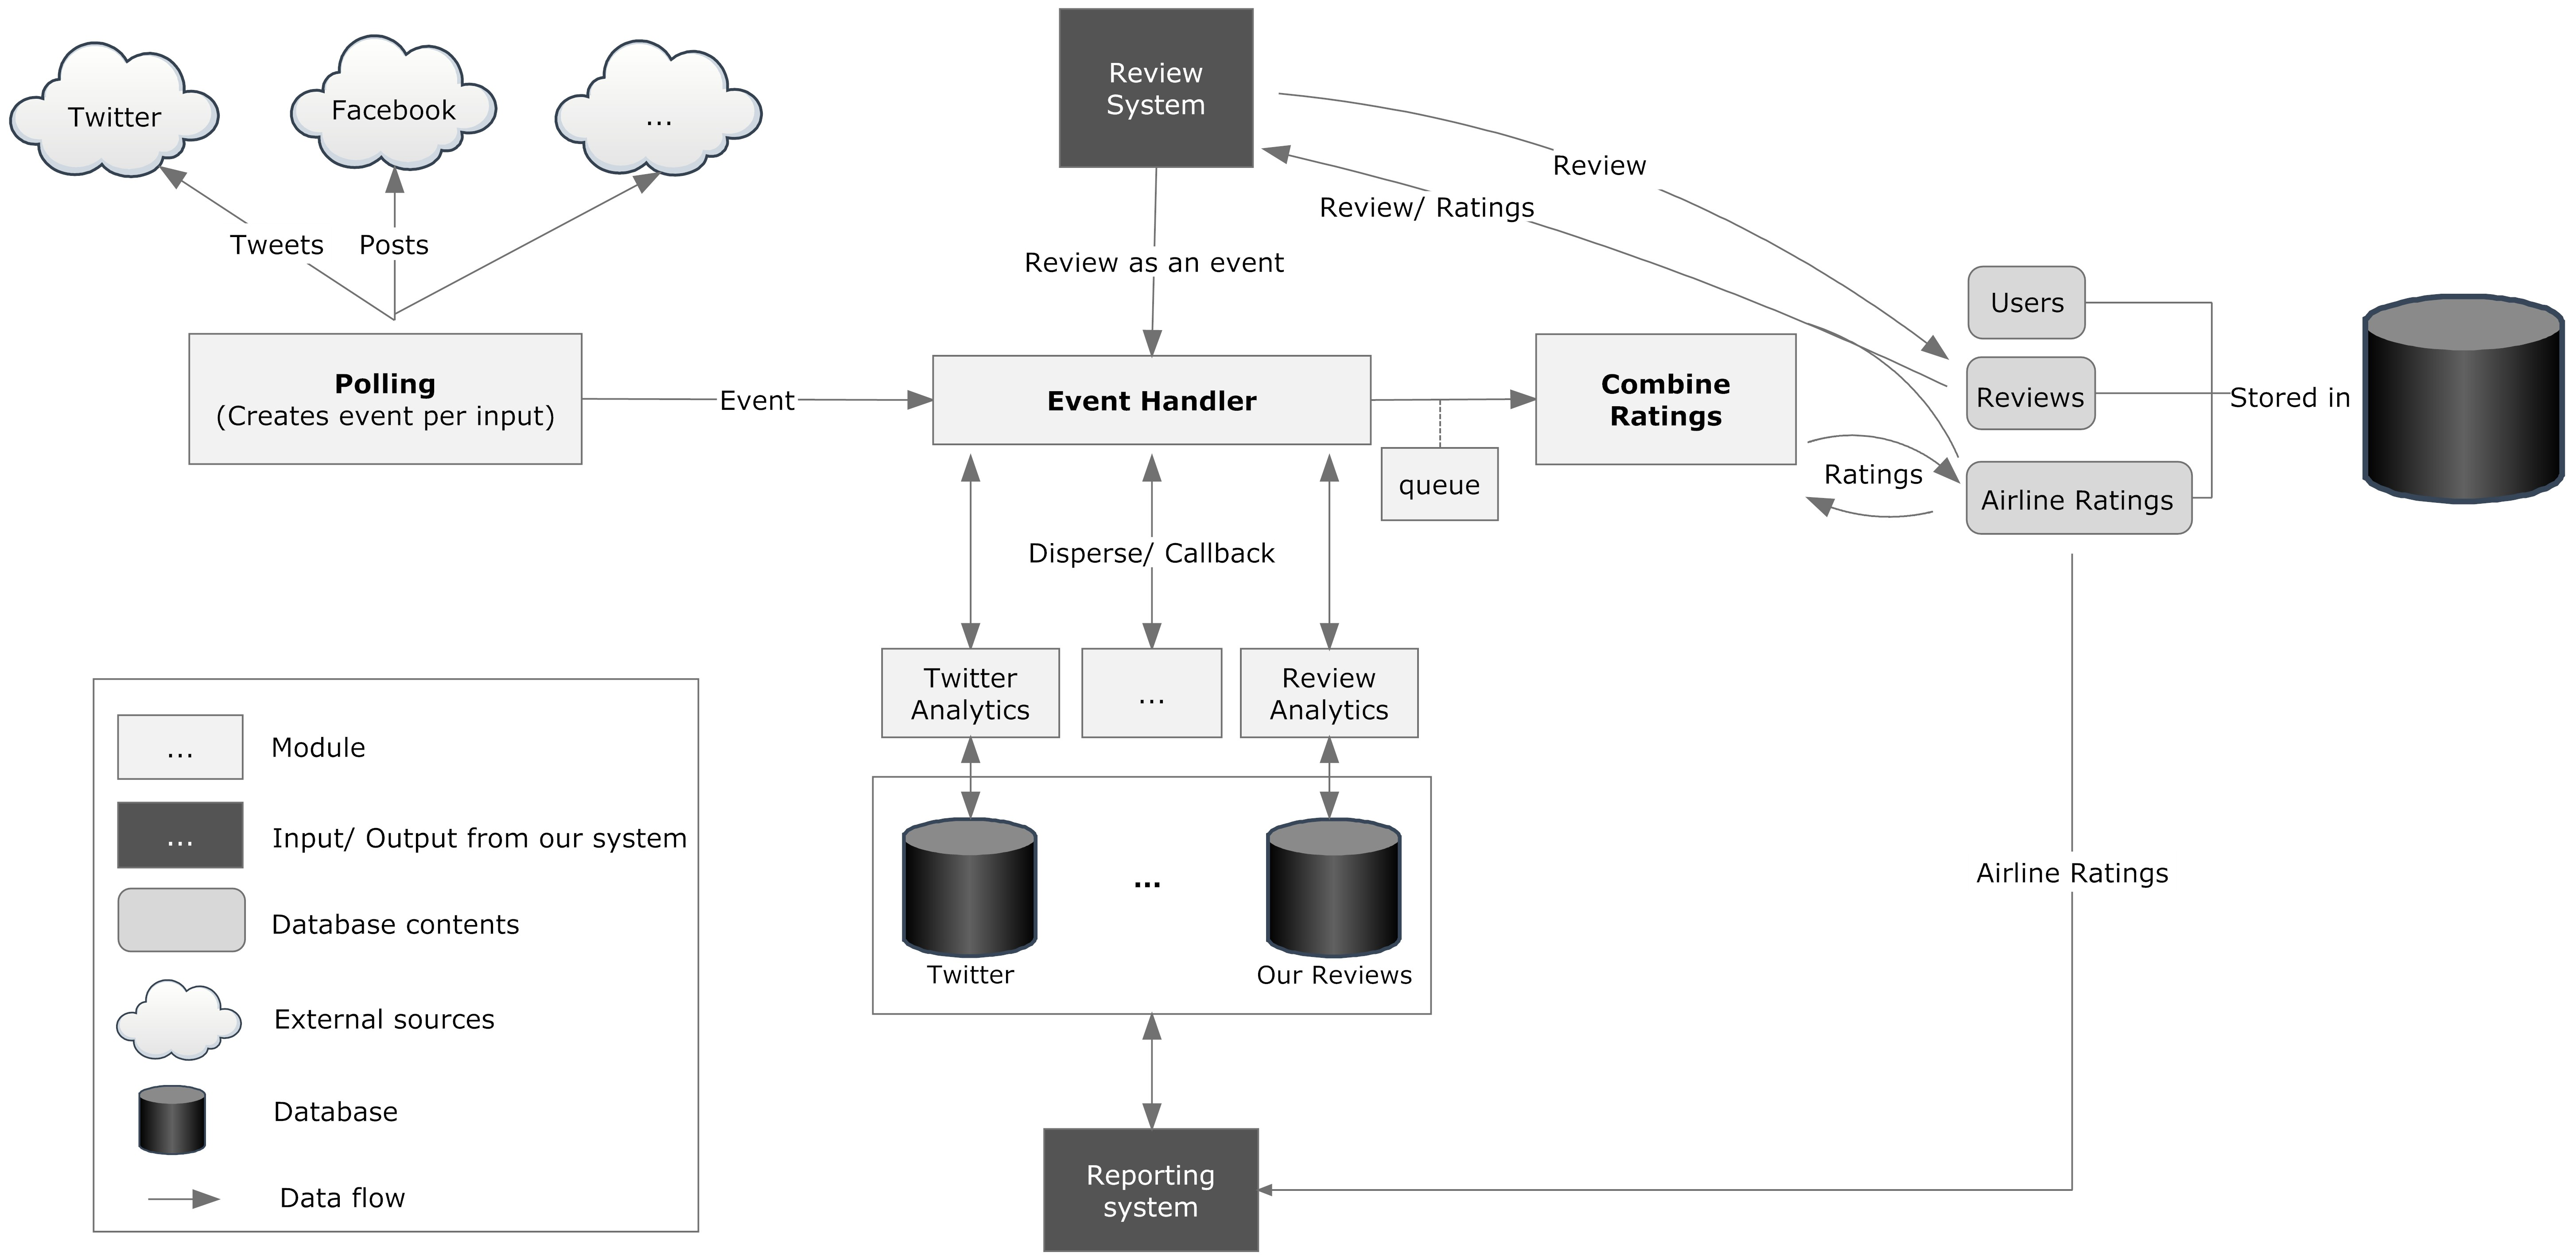
\includegraphics[width=600px]{DataFlowGraph}
\caption{Data Flow Viewpoint}
\label{fig:Data Flow}
\end{figure}
\end{landscape}

This Data Flow viewpoint \ref{fig:Data Flow} illustrates the flow of data within the back-end of the system. In this picture the review and reporting system are shown as black boxes to illustrate that their functionality is of no importance in this picture.
In the related design decisions it was argued that combining the rating with incremental updates was best for performance and scalability. Note that in the flow only the back-end of the system is given, because of the importance of handling the large data sets. Each of the modules and arrows in the viewpoint are explained here after.

\subsubsection{Polling}
The polling module is responsible for obtaining reviews from external data sources. It polls every external source on a given time-frame which is different for each external source. The reviews are not formatted and there original data format from the external source is kept. The rationale behind this decision is that all the reviews from external sources are significantly different of each other. Parsing them into a general format would lead to data loss or lots of undefined fields. The decision is further elaborated in the appendix at \ref{dd:save-raw}. The unformatted reviews are then passed on to the event handler as events. An event is defined as a single unformatted review either from external or internal sources.

\subsubsection{Event handler}
The event handler receives the events from both the polling module (external sources) and the review system (internal source). The responsibility of the event handler is to send these events to the analytics module specific to that data source. The event handler allows for parallel processing of reviews and greatly increased the performance and scalability compared to a more traditional pipeline model. This decision is further elaborated on in the appendix at \ref{dd:large-data}.

\subsubsection{Analytics}
Each data source has its own analytics module, because the data must be treated differently from external sources as they are of different format. The separate analytics modules have the added benefit of allowing for meta-analysis specific to a given data source. An example could be the amount of followers on twitter.

The analytics module analyses the unformatted review and produces a rating on a given scale for a certain or multiple categories (Overall, food, timeliness etc.). The unformatted review together with the analysed ratings are then stored in the analytics database of the data source. This is a requirement by the Initiator and KLM. The decision is further discussed in the appendix \ref{dd:data-format}. The ratings are also send of the combine ratings module in order to update the rating of the airline that is related to the review.

\subsubsection{Combine Ratings}
The combine ratings module is responsible for combining the ratings from the individual reviews into a final rating for an airline. The module receives the ratings from the analytics module and obtains the old rating from the main database. These two are combined in order to form a new rating. The process of iteratively combining ratings instead of recalculating is made for performance reasons as it is much cheaper and efficient to not recalculate the ratings that are already in the final rating of the airline. This decision is discussed in the appendix at \ref{dd:recalc-comb}. The ratings are based on an airline and a specific category (overall, timeliness, food etc.).

\subsubsection{Modules}
The functionality of each of the modules is discussed in the functional view. Hence in this section only the data flow regarding each of the modules is discussed:

\begin{enumerate}
\item \emph{R \& R module} A new review is inserted as event into the event handler which can pass it off to the specific analytics module. The decision was made to save the internal reviews twice: once in the main database and once when the they are analysed in the Analytics database. This allows the users to see the reviews without accessing the analytics database, but increases overhead as the same data is almost saved twice.
\item \emph{Reporting module} The reporting module retrieves information from the analytics database which contain all the analysed data together with the raw reviews. It must also be able to access the main database for the latest final ratings.
\item \emph{Authentication module} The user data for logging purposes is saved in the main database. The data contains sensitive information and is therefore encrypted.
\item \emph{Billing module} In order to make a profit airlines need to pay for their functionality. Therefore the billing module is able to read the current enlisted airlines and write to the database if the airlines have paid or not.
\item \emph{Messaging module} The messages are saved separately in the main database. Because they can contain user sensitive information (e.g. Flight numbers, names) the whole messages are saved in an encrypted form.
\end{enumerate}


\subsection{Data Flow Viewpoint}

\begin{itemize}
\item Related stakeholders: KLM, Initiator
\item Related Concerns: Data Integrity, Performance, Scalability
\item Related design decisions: How is the data split up into multiple databases?; How do we handle large data-sets?; Recalculate or Combine rating?; Incremental or Time-interval update?; Flight-Information
\end{itemize}

\newpage
\begin{landscape}
\begin{figure}
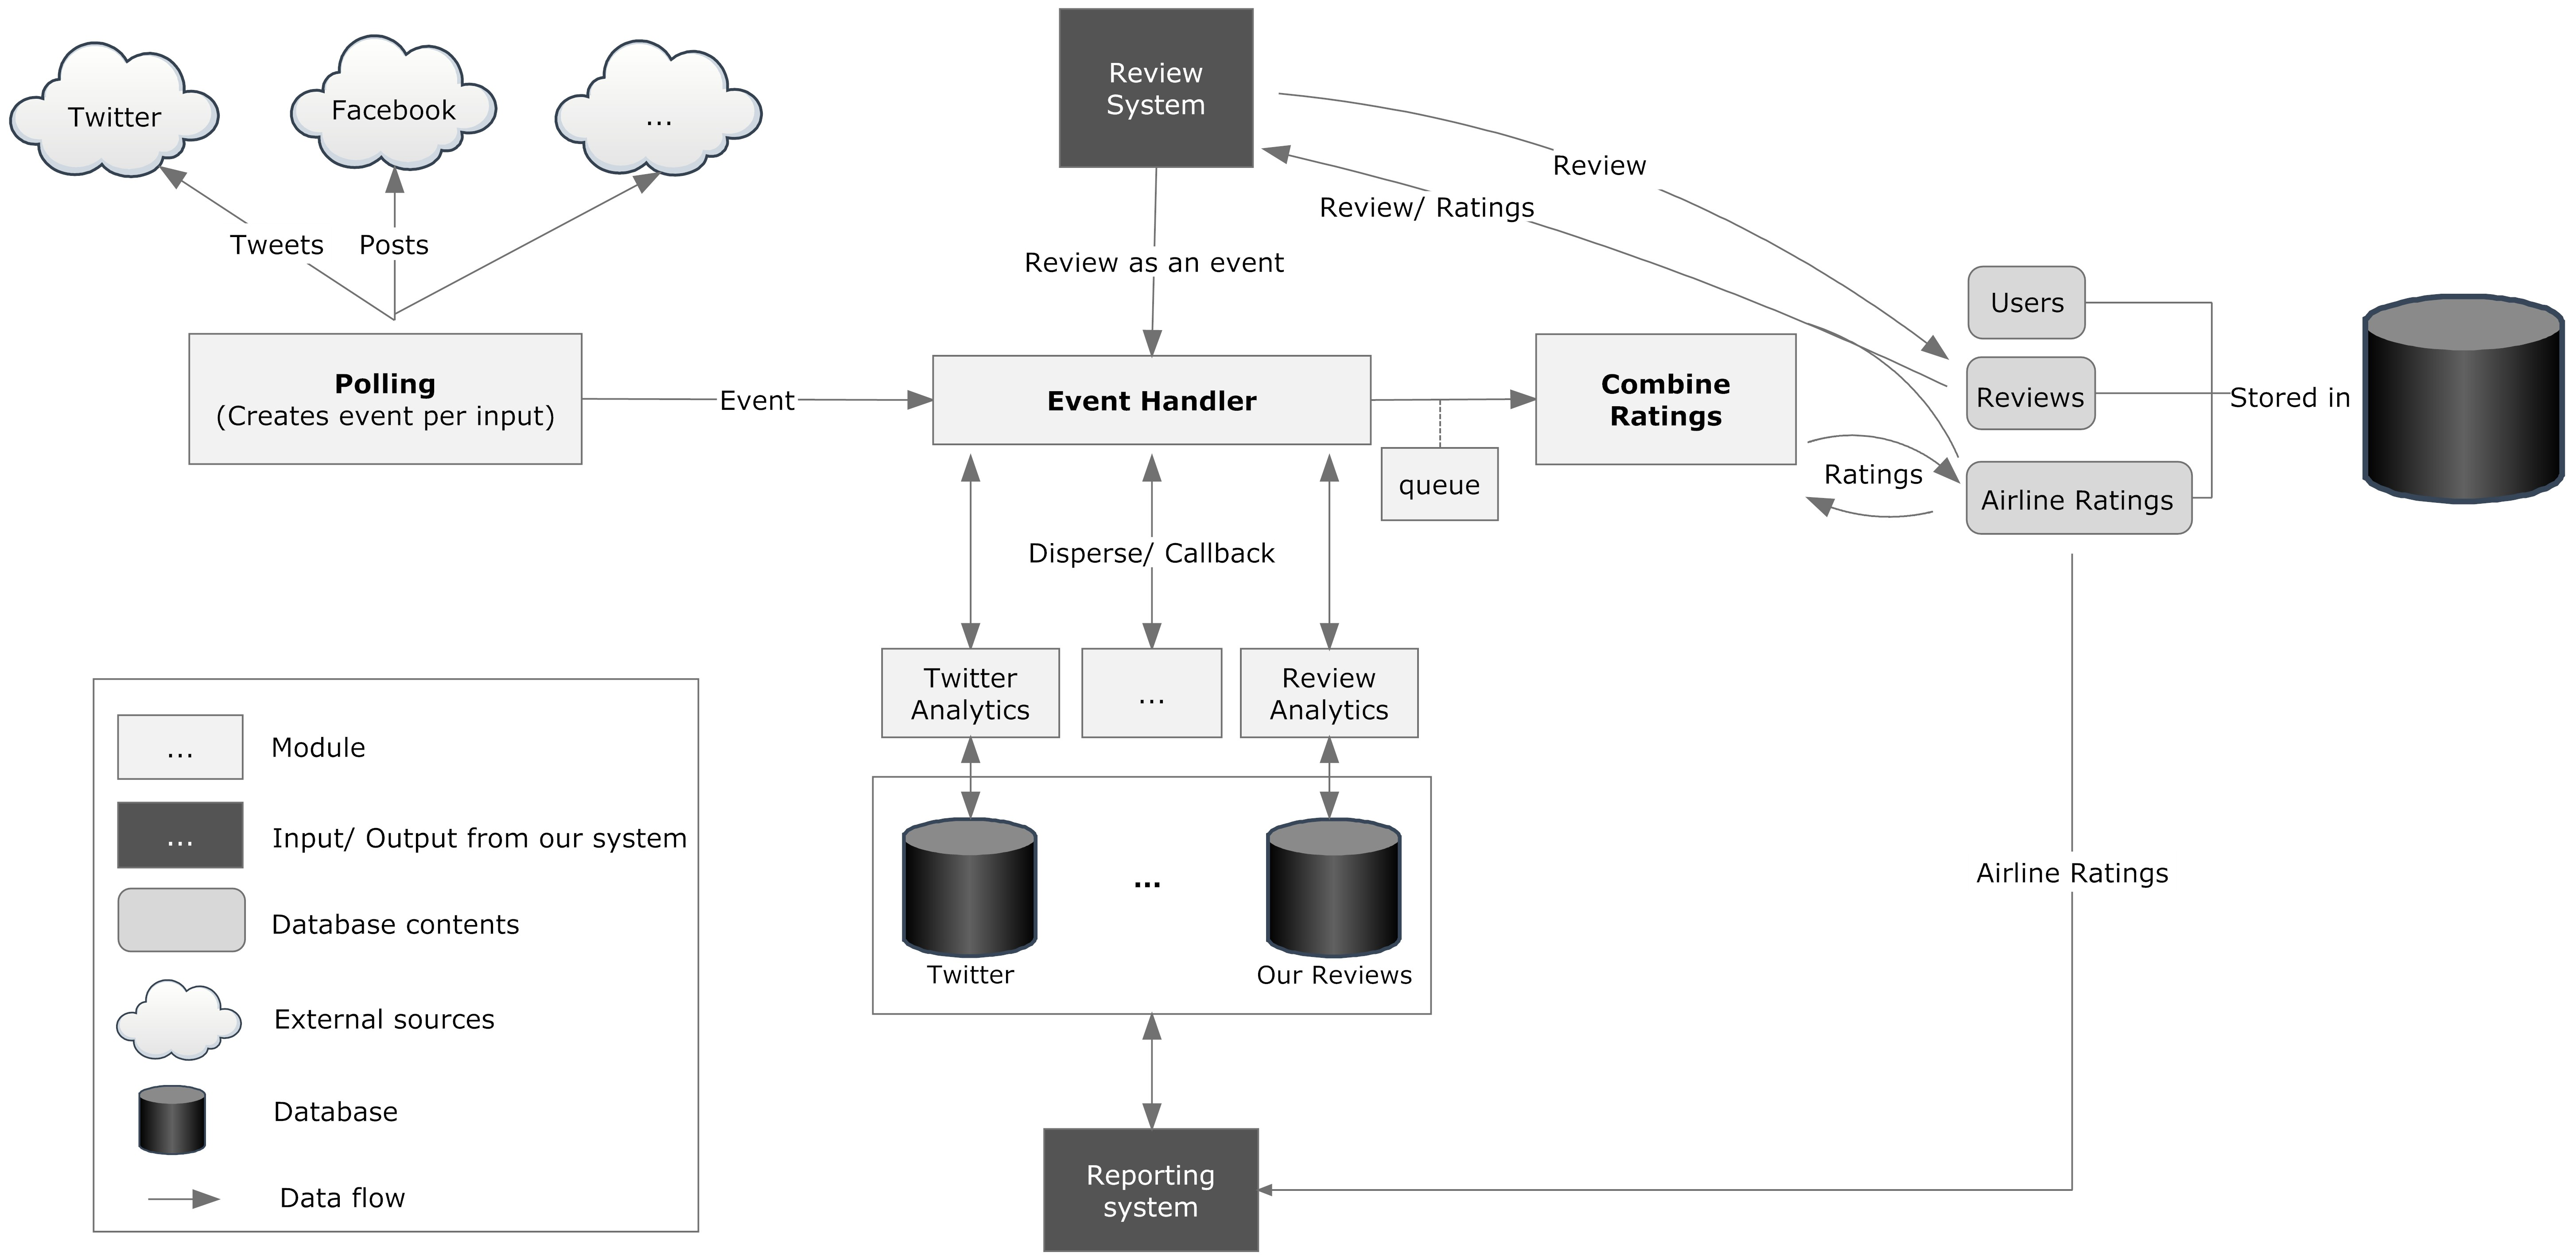
\includegraphics[width=600px]{DataFlowGraph}
\caption{Data Flow Viewpoint}
\label{fig:Data Flow}
\end{figure}
\end{landscape}

This Data Flow viewpoint \ref{fig:Data Flow} illustrates the flow of data within the back-end of the system. In this picture the review and reporting system are shown as black boxes to illustrate that their functionality is of no importance in this picture.
In the related design decisions it was argued that combining the rating with incremental updates was best for performance and scalability. Note that in the flow only the back-end of the system is given, because of the importance of handling the large data sets. Each of the modules and arrows in the viewpoint are explained here after.

\subsubsection{Polling}
The polling module is responsible for obtaining reviews from external data sources. It polls every external source on a given time-frame which is different for each external source. The reviews are not formatted and there original data format from the external source is kept. The rationale behind this decision is that all the reviews from external sources are significantly different of each other. Parsing them into a general format would lead to data loss or lots of undefined fields. The decision is further elaborated in the appendix at \ref{dd:save-raw}. The unformatted reviews are then passed on to the event handler as events. An event is defined as a single unformatted review either from external or internal sources.

\subsubsection{Event handler}
The event handler receives the events from both the polling module (external sources) and the review system (internal source). The responsibility of the event handler is to send these events to the analytics module specific to that data source. The event handler allows for parallel processing of reviews and greatly increased the performance and scalability compared to a more traditional pipeline model. This decision is further elaborated on in the appendix at \ref{dd:large-data}.

\subsubsection{Analytics}
Each data source has its own analytics module, because the data must be treated differently from external sources as they are of different format. The separate analytics modules have the added benefit of allowing for meta-analysis specific to a given data source. An example could be the amount of followers on twitter.

The analytics module analyses the unformatted review and produces a rating on a given scale for a certain or multiple categories (Overall, food, timeliness etc.). The unformatted review together with the analysed ratings are then stored in the analytics database of the data source. This is a requirement by the Initiator and KLM. The decision is further discussed in the appendix \ref{dd:data-format}. The ratings are also send of the combine ratings module in order to update the rating of the airline that is related to the review.

\subsubsection{Combine Ratings}
The combine ratings module is responsible for combining the ratings from the individual reviews into a final rating for an airline. The module receives the ratings from the analytics module and obtains the old rating from the main database. These two are combined in order to form a new rating. The process of iteratively combining ratings instead of recalculating is made for performance reasons as it is much cheaper and efficient to not recalculate the ratings that are already in the final rating of the airline. This decision is discussed in the appendix at \ref{dd:recalc-comb}. The ratings are based on an airline and a specific category (overall, timeliness, food etc.).

\subsubsection{Modules}
The functionality of each of the modules is discussed in the functional view. Hence in this section only the data flow regarding each of the modules is discussed:

\begin{enumerate}
\item \emph{R \& R module} A new review is inserted as event into the event handler which can pass it off to the specific analytics module. The decision was made to save the internal reviews twice: once in the main database and once when the they are analysed in the Analytics database. This allows the users to see the reviews without accessing the analytics database, but increases overhead as the same data is almost saved twice.
\item \emph{Reporting module} The reporting module retrieves information from the analytics database which contain all the analysed data together with the raw reviews. It must also be able to access the main database for the latest final ratings.
\item \emph{Authentication module} The user data for logging purposes is saved in the main database. The data contains sensitive information and is therefore encrypted.
\item \emph{Billing module} In order to make a profit airlines need to pay for their functionality. Therefore the billing module is able to read the current enlisted airlines and write to the database if the airlines have paid or not.
\item \emph{Messaging module} The messages are saved separately in the main database. Because they can contain user sensitive information (e.g. Flight numbers, names) the whole messages are saved in an encrypted form.
\end{enumerate}




\section{Description of our Solution}

\appendix

\section{Domain Knowledge - Design Decision}
In this section we will present the domain specific problems related to airline reputation management system. To divide the workload four separate directions were defined. These  
directions are highly interconnected and might not appear as separate in the final design. The four directions are:
\begin{enumerate}
\item User Experience
\item Competition and Functionality
\item Data storage
\item Data Gathering
\end{enumerate}
A separate section has been dedicated to each of the direction. 

\subsection{Domain Specific Problems Related to User Experience}
\subsubsection{Important Questions}
The purpose of this section is to ask domain specific question related to user experience. The interface consists of all front-end systems that are directly in contact with the users. 
In order to get a better insight over the domain we searched through websites relevant to airline companies. We tried to understand what is important to the users and what they are looking for in
a rating site. The questions that  are important to the interfaces which affect user experience are:
\begin{enumerate}
\item What types of customers are distinguished in the system?
\item What kind of interactions should each customer be able to perform?
\end{enumerate}

\subsubsection{Design Decisions}
During our meetings with the stakeholders it was made clear that there are two types of customers:
\begin{enumerate} 
\item Clients: In general, the people who write and read the reviews and ratings.
\item Business Clients: The airline companies. The airline companies want to see a general overview of their companies ratings and reviews with some additional features such as the 
reporting system (discussed in the next section)
\end{enumerate}

An overview of the functionalities available to these groups of user is described below: 
\begin{itemize}
\item Clients (Registered Users):
	\begin{enumerate}
		\item They can write ({\em anonymously}), read and vote the reviews (Review System).
        \item They can see and compare the ratings of different airline companies.
        \item They can accept the invitation of an airline based on one of their reviews to a private conversation (Messaging System). 
		\item They can Invite EU claim to a private conversation.
	\end{enumerate}
\item Business Clients (Airline Companies):
	\begin{enumerate}
		\item They can write feedback to a user's review.
		\item They can invite a user to a private conversation based on a review in order to resolve his/ her complaint.
		\item They can see the current ratings and/ or the latest (bad) reviews posted (Reporting System).
		\item They can see statistics about their progress.
		\item They can see their progress in comparison with other airline's progress (only if they share their information as well).
		\item They can insert flight information and search through our databases to find patterns.
	\end{enumerate}
\end{itemize}

The fact that these two groups have clearly different functionalities results in two options concerning the system's interface, either two totally separate sites, or a general page 
whose content will change depending on the signed in user but the lay out will be the same.

In addition to these groups there two more:
\begin{itemize}
 \item Guests: Unregistered users who can only search for airlines and read reviews and ratings.
 \item EU-Claim: EU-Claim can monitor a private conversation after a user's invitation. Furthermore, is notified if a conversation is not ''resolved'' for a specified period of time.
\end{itemize}


\subsection{Domain Specific Problems Related to Competition and Functionality}
\subsubsection{Important Questions}
The purpose of this section is to find the domain specific questions related to our functionality. To accomplish that, we searched in the internet to learn more about our competition
and what they offer in order to adapt our system's architecture to focus on the functionalities that are going to differentiate us from them. The questions that help us understand the 
domain are:
\begin{enumerate}
\item Who is our biggest competitor?
\item Do we need to handle online payment?
\item How do the feedback and the messaging systems work?
\item How will the reporting system work?
\item How can we protect our results?
\item How do we ensure the users' privacy?
\item Which features of our review format are going to ensure users' privacy?
\end{enumerate}

\subsubsection{Design Decisions}
\paragraph{Competition} Our greatest competitor seems to be http://www.airlinequality.com/. This site contains reviews about 681 airlines and 725 airports and uses a “star” rating 
system called SKYTRAX. SKYTRAX has been used since 1999 and right now seems to be the only globally accepted airline rating system (is recognized as a global benchmark for airline 
standards). Fortunately, it does not provide feedback and reporting system. Consequently it is recommended to focus these systems.

\paragraph{Online Payment} It was requested that the services to the airlines will be available after payment. The payment can either take place online or offline. In the first case, 
the stakeholders are going to have an extra cost (fee: a percent of every transaction or predefined + 10\$ – 25\$ every month). On the other hand since the 
payment is addressed only to airline companies it is possible to do that offline through contracts, invoices etc.

\paragraph{Feedback \& Messaging System} The platform of FlyWithUs provides to the airlines the opportunity to respond to a review if they believe it is necessary. (Feedback system)

Additionally, an airline will be able to invite a user to a private conversation based on bad review in order to address an issue or to try to compensate him/ her. The user can choose 
if he/ she wants to continue and if he/ she wishes to provide his/ her information.

It is also significant to decide whether preserving the integrity of the system's  messaging service is desirable. To accomplish that, EU-Claim could be able to monitor the private 
conversation. Although the user will be notified about this, it may still be against his/ her privacy. EU-Claim proposed this functionality to be available only if the user enables 
it and not by default and KLM representative and the initiator agreed as well.

Furthermore, it is desirable for such a conversation to have states for example “resolved”  and “pending”, then a user can change a its state from pending to resolved. As a result 
EU-Claim can be notified by the system if a report has been unresolved for a certain period of time.  Additionally, the state of a conversation allows us to calculate the resolved 
issues and include that result in our website in order to encourage people to use our system.

\paragraph{Reporting System} The reporting system is a functionality only available to airlines. Each airline will be able to monitor its rating status through a report webpage which will comprise of the following components:
\begin{itemize}
\item Statistics concerning its progress through graphs and diagrams.
\item Latest reviews or bad reviews from our site.
\item Cross-reference flight information with the reviews stored on our system.
\item Comparison between airlines (only if the airline shares her information also)
\end{itemize}

\paragraph{Prevent Aggregation – Copyright} The copyright of the data that will be collected should be further investigated according to the policy of each source. If the legality of 
harvesting data from the other sources is resolved and even if the data gathered are public, the collection of the data on our system can be protected. This can be achieved because 
even though the data are public a collection of them is copyrightable. Additionally, we can use a file called robots.txt to prevent data aggregation from specific crawlers. However, 
the effectiveness of this file lies entirely on the crawlers because they can ignore the file. It appears that there are no architecture relevant questions on this question.

\paragraph{Users' Privacy} As it was mentioned in the section Feedback \& Messaging Systems, users' privacy is an important issue. This issue was raised by three of the stakeholders 
Dutch government, EU-Claim and the initiator. A user's data and conversations with airlines are private, this means that these information are available only after user authentication 
and in the case of the private conversation available only to the airline of interest (maybe to EU-Claim as well if the user requests that). 

\paragraph{Review's Format} Since user's privacy is a big issue the review's format should allow anonymity. This is accomplished by omitting the name, username or any other author 
identifier from the public representation of a review.

\subsection{Domain specific problems related to data gathering and Analysis}
\subsubsection{Import questions}
The purpose of this section is to explain domain related problems related with this task. The data gathering is responsible for polling external sources and providing the data to the storage system. This implicates two important question which are further elaborated next:
\begin{enumerate}
\item	How is the data from different external sources combined?
\item	How is the combined data used in order to obtain a rating?
\item	Is there any filtering process on the external data?
\end{enumerate}
The external sources vary from airline companies sites to review sites to social networks. These all have their own way of inputting a review. For instance, Twitter does not have any format related to the review and only consists of lines text, while review sites already have  a format in place that allows the user to rate some of the attributes (Food, timeliness, service etc.) on a given scale. The final application should be able to digest all these kinds of reviews and output the results on a scale . 
A separate , however still important, question relates to the quality of the data. The external sources may or may not have systems in place that assure the quality of a review. Since the data is not inspected 

\subsubsection{Design Decisions}

\paragraph{Combining external sources}
The sources have their own unique format as explained earlier in the document. If the system where to parse this into a general format information might get lost or lot's of information is undefined.
However the general format helps decrease the complexity of analysing, because that system does not need to account for all the unique formats. This decision requires further collaboration with the data storage
as that needs to be able to handle the data. 

\paragraph{Analysing external sources}
Not all external sources give a rating on a scale (e.g. Twitter) therefore these reviews need to be analysed first in order to be useful. There are multiple options available when analysing these results:
\begin{enumerate}
\item Drop all reviews that have no rating attached to them. This would lead to a huge data loss, but decrease the complexity of the system. The ratings can then easily be combined by computing a weighted average (or by another formula) of the individual ratings.
\item Transform the reviews without ratings by performing a sentiment analysis. After the analysis the ratings can be combined the same as in the other option.
\end{enumerate}

\paragraph{Filtering}
Some reviews may not be considered useful, because of certain properties. The system could apply some business rules in order to filter those reviews out. The business rules governing these reviews are however currently unknown. 




\subsection{Domain specific problems related to data storage}
\subsubsection{Import questions}
This section lays out the domain related questions with data storage. The system is responsible for storing several kinds of data both from the local system as well as data from external sources. This implies several questions:
\begin{enumerate}
\item What kind of data does the system need to store?
\item How big is the data from external sources?
\item How does the system read and write the different data types?
\end{enumerate}
The system has to store information such as users, reviews, statistics, data from external sources, etc. Because of the variety of data types it is important to understand these data types and how the system utilizes this data.

The data categories we define are:
\begin{enumerate}
\item Users: The system requires a user management system to log in and out on the web application. This user data needs to be stored persistently. An important quality attribute related to this user data is privacy, because it holds sensitive information.
\item Reviews: The users should be able to read and write reviews on the website.
\item Data from data-mining: The polling module (discussed previously) supplies the system with data from different external sources (e.g. Tripadvisor, Twitter). Because of the large amount of data scalability is a key quality attribute.
\item Analysis results: The data from external sources is analysed to form a rating and calculate statistics for the airline companies. Performance is a key quality attribute here as these results are shown to a potentially large number of end users, as well as scalability as the statistical data grows fast over time.
\end{enumerate}

To get an idea of the amount of data we get from external sources, we use the following number. There currently exist over 600 airline companies. To calculate values for 600 companies we take one specific company (KLM) and multiply the values found for this company with 600:
\begin{enumerate}
\item Twitter: There are 1.4 Tweets per minute on KLM. This would indicate that there are approximately 600 * 1.4 * 60 * 24 = 1.008.000 tweets per day on airline companies
\item Facebook: There are 101277 talking about KLM on Facebook. This would indicate that in total 60.766.200 posts are about airline companies
\item Tripadvisor: There are currently 470 reviews on KLM. This indicates that there are 282.000 reviews on airline companies.
\end{enumerate}
The size of the data already shows that great care must be taken in the data-mining and analysis step regarding to performance and as new external sources may be added over time, scalability is also of great importance.


\subsubsection{Design Decisions}
\paragraph{One or more databases?}
The system has to handle data from multiple sources and different usage types. For instance, the data-mining and statistics require a lot of write commands as opposed to reads, whereas the main website data, such as reviews and users, requires more read commands as opposed to writes. For this reason the usage of specialized databases for each would increase performance and scalability.

\paragraph{How many databases?}
If we use more than one database we need to decide how much we can split up the data while still keeping it maintainable.
A this time we have several options:
\begin{enumerate}
\item Split up the main website data and data extracted from data-mining.
\item Split up the main website data, data-mining data and statistical data.
\item Split up the main website data and for each external source have a separate database containing the data-mined data.
\end{enumerate}

\paragraph{How do we handle large data-sets?}
The data collected from external sources require a great amount of storage over time. In addition to that, all the incoming data has to be analysed to create new ratings and statistical data. For this data both performance and scalability are the most important attributes.
By utilizing an event type system we can balance the load and only write away data after it has been analysed, thus decreasing the amount of reads and writes the database has to run. The implication is that data in the event handler/queue is not persistent to the database and may be lost in system failures.

\paragraph{Always recalculate ratings or combine with the known value?}
When new data is collected from external sources or when a review is made, the rating for the airline company needs to be updated. While a complete recalculation allows you to always change the weight of your external sources and reviews, it also means that over time more and more data has to be read from the database. Because of that the performance will deteriorate over time.
To prevent this from happening, utilizing known values can greatly improve performance. By keeping track of the amount of tweets/reviews/etc received and the current rating, you only add the new input to those values by calculating the weight and the share it has on the total. By doing so you don't traverse the whole database thus greatly improving performance. If a recalculation is required this could always be initiated separately.

\paragraph{Incremental or time-interval updates?}
When new data is received, the rating and statistics need to be updated. This can either be done on a time-interval, such as once an hour, or using a queue and continuously update the data. To get the best performance and to safe on hardware cost, the latter is the most optimal solution. By spreading out the load, the machine does not need to handle high peaks and therefore you don't need to have a machine build to handle the peak when it happens. This means that the system required to run the updates can be run on a less powerful system thus saving cost. It also means that the data is always being updated and that the users get the most recent information possible.

\paragraph{Flight-data usage}
The stakeholder interest in flight-data was the decreasing of the weight of ratings during delays caused by things out of the hands of the company, such as bad weather, and to see a relation in the statistics between flight-data and the height of their rating. To ensure the integrity of the reviews and to improve the performance of the system, we advice against the use of flight-data to decrease the weight of reviews. By doing so we don't have to read from the database to get the flight-data to filter reviews thus saving resources and gaining performance. It also ensures the data integrity as it may be possible that flight-data is entered after bad reviews have already been added to the system. It is also the case that if a flight is delayed or cancelled the service from the airline company to accommodate the passengers is being put to the test. This should not be weighted less because the flight-data says the delay is due to bad weather.



\begin{thebibliography}{9}

\bibitem{clemens}
Bass et al.
  \emph{Software Architecture in Practice}.
  Addison Wesley, Boston,
  3rd Edition,
  2012.

\bibitem{hayesroth}
 Hayes-Roth, F
 \emph{Architecture-Based Acquisition and Development of Software: Guidelines and Recommendations from the ARPA Domain-Specific
 Software Architecture (DSSA) Program},
 Teknowledge Federal Systems,
 1994

\bibitem{IEEE1471}
 IEEE Std 1471-2000,
 \emph{Recommended Practice for Architecture Description of Software-Intensive Systems},
 United States,
 2000

\bibitem{lane90}
  Lane, Thomas,
  \emph{Studying Software Architecture Through Design Spaces and Rules}.
  Software Engineering Institute, Carnegie Mellon University,
  1990.

\end{thebibliography}

\end{document}

